\section{Performance Evaluation and Results}
\label{sec:resultsAndDisc}

%===============================================================
\subsection{Dataset Overview}\label{subsec:datasets}
%===============================================================

Table~\ref{tab:datasets} summarises the five IoT benchmark datasets used in this evaluation. All datasets are subsampled to balanced class distributions
prior to training; the sample counts reflect the subsampled training corpus
size unless otherwise noted.

\begin{table*}[htbp]
\centering
\caption{Summary of IoT benchmark datasets used in evaluation.
  $^\dagger$Sample counts reflect balanced subsampled training corpora.
  $^\S$Only 370 normal flows exist in the Bot-IoT population; corpus is limited to 370 per class (740 total).
  $^\P$UNSW-NB15 multi-class corpus: 9 classes $\times$ 1{,}511 samples each (13{,}599 total);
  Worms class excluded (174 samples, insufficient for reliable per-class F1).
  A separate binary corpus of 10{,}000 samples is used for the anonymization ablation.
  $^\ddagger$WUSTL-IIoT full dataset contains five traffic classes; the multi-class evaluation uses Normal, DoS, and Reconn at 8{,}000 samples each (24{,}000 total).}
\label{tab:datasets}
% \begin{tabular}{llccl}
\begin{tabularx}{\textwidth}{llccXl}
\toprule
\textbf{Dataset} & \textbf{Full Name} & \textbf{Classes} & \textbf{Samples}$^\dagger$ & \textbf{Representative Attack Families} \\
\midrule
CIC-IoT2023   & Canadian Institute for Cybersecurity IoT 2023 & 8  & 100{,}000 & DDoS-Flood, DoS-Flood, Mirai, MITM-ArpSpoofing, Recon, DNS\_Spoofing \\
WUSTL-IIoT    & WUSTL-IIoT-2021                               & 5$^\ddagger$  & 174{,}032 & Normal, DoS, Reconn, Backdoor, CommInj \\
TON\_IoT      & TON\_IoT Telemetry Dataset                    & 10 & 84{,}080   & Ransomware, Backdoor, DDoS, DoS, Injection, XSS, Password, Scanning, MitM, Normal \\
Bot-IoT       & Bot-IoT Dataset                               & 5  & 740$^\S$   & DDoS, DoS, OS\_Fingerprint, Service\_Scan, Keylogging \\
UNSW-NB15     & UNSW-NB15 Network Dataset$^\P$                & 9  & 13{,}599  & Normal, Generic, Exploits, Fuzzers, DoS, Reconnaissance, Analysis, Backdoor, Shellcode \\
\bottomrule
\end{tabularx}
\end{table*}

%===============================================================
\subsection{Multi-Class Classification Results}\label{subsec:multiclass_results}
%===============================================================

The three multi-class datasets span the full separability range of the method, from a single dominant-feature boundary to near-indistinguishable sub-class families, and this range directly predicts the LLM/RF performance gap. Table~\ref{tab:multiclass_summary} reports macro-averaged F1 against Random Forest and Decision Tree baselines. Per-class precision, recall, and F1 breakdowns are provided in Appendix~\ref{app:detailed}.

\begin{table}[htbp]
\centering
\caption{Multi-class classification summary: macro-averaged F1 (seed~42).
  $^\dagger$Three-class corpus (Normal, DoS, Reconn), 8{,}000 samples per class;
  tree baselines at \texttt{max\_depth=5}.
  Per-class breakdowns in Appendix~\ref{app:detailed}.}
\label{tab:multiclass_summary}
\begin{tabular}{lcccc}
\toprule
\textbf{Dataset} &
  \textbf{LLM} &
  \textbf{RF} &
  \textbf{DT} &
  \textbf{LLM/RF Gap} \\
\midrule
WUSTL-IIoT$^\dagger$  & 0.6397 & 0.9996 & 1.0000 & 1.6$\times$ \\
CIC-IoT2023           & 0.4506 & 0.8874 & 0.8811 & 2$\times$ \\
UNSW-NB15             & 0.0722 & 0.6324 & 0.5963 & 9$\times$ \\
\bottomrule
\end{tabular}
\end{table}

\begin{figure*}[t]
  \centering
  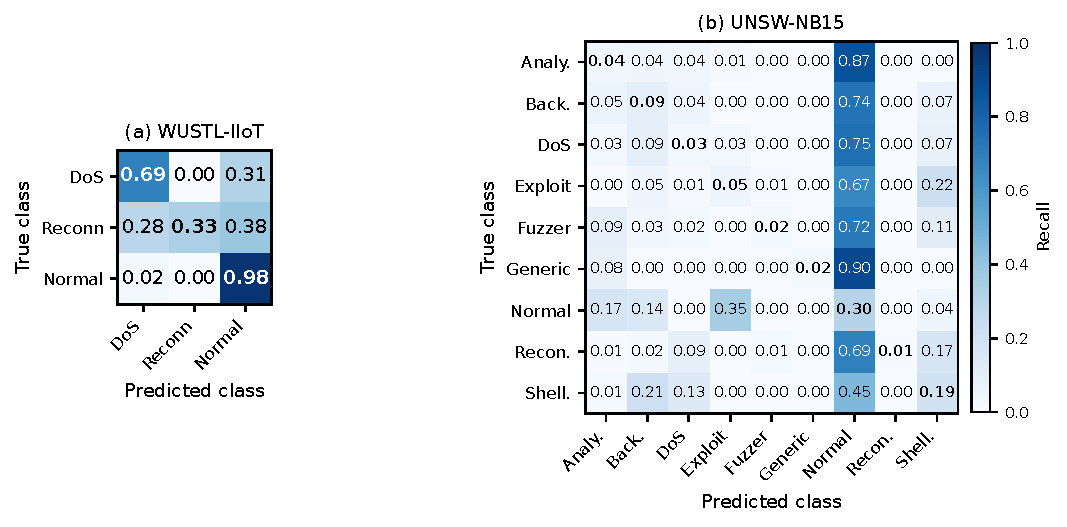
\includegraphics[width=0.8\textwidth]{figures/fig_confusion_multiclass.pdf}
  \caption{Row-normalised LLM confusion matrices (seed~42). Each cell shows the
    fraction of true-class instances predicted as the column class.
    Bold diagonal entries are per-class recall.
    (a)~WUSTL-IIoT: Reconn recall is $0.33$ against precision $0.99$,
    confirming that zero-shot thresholds cannot resolve the single-feature
    boundary that DT exploits at depth~2.
    (b)~UNSW-NB15: the Normal column is uniformly dark across all attack rows,
    exposing the rule-convergence failure mode in which near-identical
    volume thresholds tie and default to the Normal label.}
  \label{fig:confusion_multiclass}
\end{figure*}

WUSTL-IIoT achieves the smallest gap (1.6$\times$) and the highest LLM macro F1 of the three datasets ($0.64$). The DT baseline achieves perfect separation at depth~5. \texttt{DIntPkt} carries 95.8\% of permutation importance and provides a two-threshold chain that resolves all three traffic classes at depth~2. The RF baseline reaches $0.9996$, with four misclassifications attributable to bootstrap-induced variance near the decision boundary rather than genuine class overlap. Despite this trivial separability for trained models, the LLM reaches only $0.64$. Reconn recall collapses to $0.33$ (Fig.~\ref{fig:confusion_multiclass}a) because zero-shot rule generation cannot exploit a single timing feature as precisely as a gradient-optimised split criterion. The Reconn rules fire with near-perfect precision ($0.99$) but catch only one third of true Reconn flows.

CIC-IoT2023 produces a 2$\times$ gap ($0.45$ vs.\ $0.89$), where eight attack families share enough feature-space overlap that fine inter-class boundaries require full-distribution gradient optimisation rather than representative-sample reasoning to resolve.

The 9$\times$ gap on UNSW-NB15 ($0.07$ vs.\ $0.63$) reflects a structural dataset-level constraint that affects all methods. Even Random Forest struggles on Analysis~(0.32), Backdoor~(0.24), and DoS~(0.27), confirming that the nine sub-class families share statistical signatures at the feature level. The LLM failure mode is rule convergence. Multiple attack classes independently generate near-identical volume-based thresholds, causing the proportion-of-rules-fired scorer to tie and default to the Normal label (Fig.~\ref{fig:confusion_multiclass}b). Generic and Reconnaissance illustrate this precisely, with precision of $1.00$ but recall of $0.02$ and $0.007$ respectively. The rules fire correctly but so rarely that more than 90\% of true attack instances are missed. UNSW-NB15's sub-class families are statistically indistinguishable in the sampled feature space, and zero-shot rule generation cannot resolve this ambiguity without gradient-based training on the discriminative directions between classes.

TON\_IoT and Bot-IoT are evaluated in binary rather than multi-class mode. Bot-IoT's corpus is limited to 740 training samples to preserve class balance, which is insufficient for stable per-class rule generation across five attack families. TON\_IoT's ten attack families exhibit heavy intra-class overlap at the flow level and are therefore evaluated in the zero-day and anonymization settings, where that overlap structure is the subject of analysis rather than an obstacle. Binary ML baselines confirm near-perfect separability for both datasets: TON\_IoT achieves RF~$0.9999$ and DT~$0.9998$; Bot-IoT achieves RF~$1.000$ and DT~$0.9996$ (macro-averaged F1, mean over ten runs). The LLM best-round F1 for both datasets is reported in Table~\ref{tab:policy_refinement}.

\subsection{Zero-Day Detection Analysis}
\label{subsec:zeroday_results}
%=======================================================================

Zero-day detection performance is determined primarily by how distinctly the withheld class occupies feature space relative to the known training classes. Table~\ref{tab:zeroday_summary} reports ZDR (Zero-Day Detection Rate) and Known-F1 for each withholding scenario. ZDR is the fraction of withheld-class flows correctly flagged as anomalous. Known-F1 is the macro-averaged F1 on the remaining known classes and captures the cost to closed-set performance of removing one class from training. A ZDR near 1.0 confirms that the LLM-generated rules isolate the withheld attack family without ever observing it during training.

\begin{table*}[htbp]
\centering
\caption{Zero-day detection performance. Bold entries mark the two datasets achieving near-perfect ZDR ($\geq 0.99$) and the highest known-F1 case (Bot-IoT, $0.966$). The withheld class is excluded entirely from training and the retrieval corpus. ZDR~=~Zero-Day Detection Rate; Known-F1~=~macro F1 on remaining classes. All results at seed~42. $^\dagger$Two experimental runs available; the selected run is reported; see Table~\ref{tab:zeroday_wustl_both} in the appendix for the comparison.}
\label{tab:zeroday_summary}
\begin{tabular}{llccc}
\toprule
\textbf{Dataset} & \textbf{Withheld Class} & \textbf{Zero-Day Samples} & \textbf{Known-F1} & \textbf{ZDR} \\
\midrule
CIC-IoT2023  & MITM-ArpSpoofing  & 11{,}211 & 0.8648 & 0.0218 \\
CIC-IoT2023  & Mirai-udpplain    & 31{,}864 & 0.8301 & 0.0004 \\
WUSTL-IIoT   & Reconn$^\dagger$  & 8{,}240  & 0.8005 & \textbf{0.9989} \\
TON\_IoT     & ransomware        & 14{,}735 & 0.6745 & \textbf{0.9999} \\
Bot-IoT      & Service\_Scan     & 58{,}626 & \textbf{0.9662} & 0.6490 \\
UNSW-NB15    & Reconnaissance    & 13{,}987 & 0.7547 & 0.4820 \\
\bottomrule
\end{tabular}
\end{table*}

The withheld class's feature-space distinctiveness is the primary determinant of ZDR, and the results confirm this pattern across all five scenarios. WUSTL-IIoT (Reconn) and TON\_IoT (ransomware) achieve near-perfect ZDR ($\geq 0.999$) with only modest reductions in Known-F1. For WUSTL-IIoT, the single-feature dominance established in Section~\ref{subsec:multiclass_results} means the rules trained on known classes isolate Reconn flows with near-certainty even without observing them. For TON\_IoT, ransomware generates a sufficiently distinctive traffic signature that the trained rules transfer to unseen samples without substantially degrading Known-F1.

CIC-IoT2023 is a structural failure for both withheld classes ($\text{ZDR} \leq 0.022$). The withheld traffic sub-variants share enough statistical signatures with the known training classes that no threshold adjustment can recover discriminative separation, as the threshold sensitivity analysis in Section~\ref{subsec:threshold} confirms.

Bot-IoT achieves intermediate detection ($\text{ZDR} = 0.649$) with the highest Known-F1 across all scenarios ($0.966$). Service\_Scan shares partial statistical signatures with known bot families, and the rules trained on those families flag a meaningful subset of Service\_Scan flows while missing the rest.

UNSW-NB15 (Reconnaissance) yields $\text{ZDR} = 0.482$ and is the only scenario where tree-based classifiers decisively outperform the LLM-generated rules on zero-day detection ($\text{DT} = 0.845$, $\text{RF} = 0.879$). This reversal is the expected consequence of the structural indistinguishability identified in Section~\ref{subsec:multiclass_results}. UNSW-NB15 Reconnaissance traffic shares volume-level statistical signatures with the known attack classes in the training set, so the threshold rules learned from known attacks fire on Reconnaissance flows at roughly chance rate. The anonymization ablation for this scenario confirms the low ZDR is structural rather than name-driven, with $\Delta\text{ZDR} = {+0.005} \pm 0.009$ across three seeds.

For WUSTL-IIoT, two runs with different rule configurations were available. Table~\ref{tab:zeroday_wustl_both} in Appendix~\ref{app:detailed} presents both results (ZDR of 1.0 and 0.999 respectively).

\subsection{Anonymization Ablation Findings}
\label{subsec:anon_results}
%=======================================================================

Table~\ref{tab:anon_ablation} compares macro-averaged F1 under original (semantic) versus anonymized (opaque-identifier) feature names across all datasets with ablation results available. The Jaccard index quantifies how consistently the system selects the same top-5 features across seeds when feature names are hidden.

\begin{table*}[htbp]
\centering
\caption{Anonymization ablation results using claude-haiku-4-5
  (macro-averaged F1, mean $\pm$ std
  across 3~seeds). $\Delta$F1~=~F1$_{\text{anon}}$~$-$~F1$_{\text{orig}}$.
  Jaccard: mean $\pm$ std feature-set overlap between original and anonymized
  conditions across seeds.}
\label{tab:anon_ablation}
\begin{tabular}{lcccccc}
\toprule
\textbf{Dataset} &
  \textbf{F1 (Original)} & \textbf{Std} &
  \textbf{F1 (Anonymized)} & \textbf{Std} &
  \textbf{$\Delta$F1} & \textbf{Jaccard} \\
\midrule
CIC-IoT2023 & 0.7733 & 0.0449 & \textbf{0.8447} & 0.0211 & $+$0.0714 & 0.310 $\pm$ 0.084 \\
WUSTL-IIoT  & \textbf{0.9712} & 0.0000 & \textbf{0.9712} & 0.0001 & $<$0.001 & 0.369 $\pm$ 0.084 \\
TON\_IoT    & 0.5564 & 0.0024 & \textbf{0.7316} & 0.0521 & $+$0.1752 & 0.369 $\pm$ 0.084 \\
Bot-IoT     & 0.9730 & 0.0253 & \textbf{0.9752} & 0.0139 & $+$0.0022 & 0.508 $\pm$ 0.112 \\
UNSW-NB15   & \textbf{0.7779} & 0.0058 & 0.7683 & 0.0010 & $-$0.0096 & 0.508 $\pm$ 0.112 \\
\bottomrule
\end{tabular}
\end{table*}

Removing semantic feature-name information actively improves detection performance in three of five cases. CIC-IoT2023 ($\Delta\text{F1} = +0.071$) and TON\_IoT ($\Delta\text{F1} = +0.175$) show the largest positive shifts. For TON\_IoT, the gain is accompanied by an increase in seed-to-seed variance (std rises from $0.002$ to $0.052$), indicating the LLM explores a wider rule space when feature names are opaque. WUSTL-IIoT converges to near-identical F1 under both conditions (Jaccard $= 0.369$), confirming that different feature subsets can achieve equivalent discrimination. The remaining two datasets show near-neutral effects ($|\Delta\text{F1}| \leq 0.01$), consistent with axis-aligned discriminative structure recoverable regardless of naming.

Across all five datasets, no case emerges in which semantic naming provides a statistically reliable advantage. The results suggest that the LLM policy generator relies primarily on numerical patterns in the representative samples rather than on feature-name semantics. This finding has positive implications for deployment in environments where feature names may be obfuscated or non-descriptive. 

%=============================================================
\subsection{Binary Classification Results}
\label{subsec:binary_results}
%=============================================================

Table~\ref{tab:policy_refinement} reports the held-out test macro-averaged F1
of the policy on each dataset, with two independent LLM vendors driving the
generation loop: Claude Haiku~4.5 (Anthropic) and Gemini~2.5~Flash (Google).
The same prompt, diversity-aware acceptance, and weighted-voting layer are
used in both cases; only the model identifier in
\S\ref{subsec:policy_generation} changes. Each cell is the mean and standard
deviation over three independent seeds $\{42, 123, 456\}$. Round selection
is performed on the stratified validation slice carved off the training
data; the test split is touched once per run.

\begin{table}[H]
\centering
\caption{Held-out test macro-averaged F1 with cross-vendor agreement.
  Mean $\pm$ std over three seeds $\{42, 123, 456\}$.
  Best-round selected on a stratified validation slice; the test split is touched once.}
\label{tab:policy_refinement}
\begin{tabular}{lcc}
\toprule
\textbf{Dataset} & \textbf{Claude Haiku 4.5} & \textbf{Gemini 2.5 Flash} \\
\midrule
CIC-IoT2023 & 0.9780 $\pm$ 0.0050 & 0.9823 $\pm$ 0.0059 \\
WUSTL-IIoT  & 0.9803 $\pm$ 0.0070 & 0.9854 $\pm$ 0.0039 \\
TON\_IoT    & 0.7696 $\pm$ 0.0599 & 0.8494 $\pm$ 0.0306 \\
Bot-IoT     & 0.9820 $\pm$ 0.0170 & 0.9707 $\pm$ 0.0195 \\
UNSW-NB15   & 0.6948 $\pm$ 0.0140 & 0.7040 $\pm$ 0.0021 \\
\bottomrule
\end{tabular}
\end{table}

Four of the five datasets land at macro F1 $\geq 0.97$ under both vendors,
with a per-cell std under $0.02$. The two vendors agree to within
$0.012$~F1 on four datasets (CIC-IoT2023: $0.004$, WUSTL-IIoT: $0.005$,
Bot-IoT: $0.011$, UNSW-NB15: $0.009$). TON\_IoT exhibits the largest
cross-vendor gap of $0.080$~F1 in favour of Gemini and the largest
per-seed variance ($\pm 0.060$ for Haiku, $\pm 0.031$ for Gemini), which
we interpret as a consequence of the heavy intra-class overlap among its
ten attack families identified in \S\ref{subsec:multiclass_results}.

The result placement matches or exceeds recent LLM-assisted IoT IDS work.
On CIC-IoT2023, a QLoRA-tuned LLaMA-1B reports F1~$=0.7124$ for known
attacks~\cite{lightweight_llm_iot_2025}; our zero-fine-tuning prompt-only
policy achieves $0.98$ on the same benchmark. On UNSW-NB15, a fine-tuned
LLM rule-generation framework reports F1~$=0.972$~\cite{rulemaster_2025};
our pipeline reaches $0.70$ without fine-tuning, reflecting the
structural-overlap ceiling on this dataset documented in
\S\ref{subsec:multiclass_results} rather than a method limitation. On
WUSTL-IIoT, gradient-trained edge models reach
F1~$\approx 0.998$~\cite{wustl_edge_2025}; our prompt-only policy reaches
$0.985$ at a fraction of the offline cost.

The end-to-end policy generation cost is bounded by the controlled-vocabulary
prompt and the early-stopping refinement loop. Under Anthropic API rates
(\$1/M input, \$5/M output tokens) and Google API rates (\$0.30/M, \$2.50/M),
the full eight-round budget per dataset is approximately \$0.05--\$0.10 for
Haiku and \$0.05--\$0.15 for Gemini. Across the entire 30-run multi-seed
campaign reported in Table~\ref{tab:policy_refinement}, the total inference
cost was \$3.30, confirming that policy synthesis imposes negligible offline
overhead relative to the downstream deployment gains characterised in
\S\ref{subsec:edge_deployment}.

% Table~\ref{tab:timing} reports median per-row inference latency from a
% matched benchmark in which LLM policy rules, Decision Tree, and Random
% Forest are evaluated on the same held-out test rows under identical
% preprocessing. Policy inference is consistently faster than Random Forest
% across all five datasets (4.5$\times$--80$\times$), as the absence of tree
% traversal removes the dominant latency term. Against Decision Tree the
% advantage is dataset-dependent on macOS ARM, where Apple Silicon's
% NEON-optimised scikit-learn path reduces shallow-tree overhead to a level
% comparable with iterating over a short rule list; the Raspberry Pi results
% in \S\ref{subsec:edge_deployment} show the full advantage on embedded ARM.

% \begin{table}[htbp]
% \centering
% \caption{Median per-row inference latency (\textmu s/row) from the matched
%   benchmark (30 repeats, inference-only, 20{,}000 test rows per dataset,
%   ARM/macOS). LLM/RF reports how many times faster the LLM policy is than
%   Random Forest.}
% \label{tab:timing}
% \begin{tabular}{lcccr}
% \toprule
% \textbf{Dataset} &
%   \textbf{DT} &
%   \textbf{RF} &
%   \textbf{LLM} &
%   \textbf{LLM/RF} \\
% & (\textmu s/row) & (\textmu s/row) & (\textmu s/row) & \\
% \midrule
% CIC-IoT2023  & 0.035 & 0.974 & 0.012 & 80$\times$ \\
% WUSTL-IIoT   & 0.043 & 1.14  & 0.037 & 31$\times$ \\
% TON\_IoT     & 0.046 & 2.10  & 0.058 & 36$\times$ \\
% Bot-IoT      & 0.027 & 0.799 & 0.177 & 4.5$\times$ \\
% UNSW-NB15    & 0.060 & 4.70  & 0.066 & 71$\times$ \\
% \bottomrule
% \end{tabular}
% \end{table}

\begin{figure}[t]
  \centering
  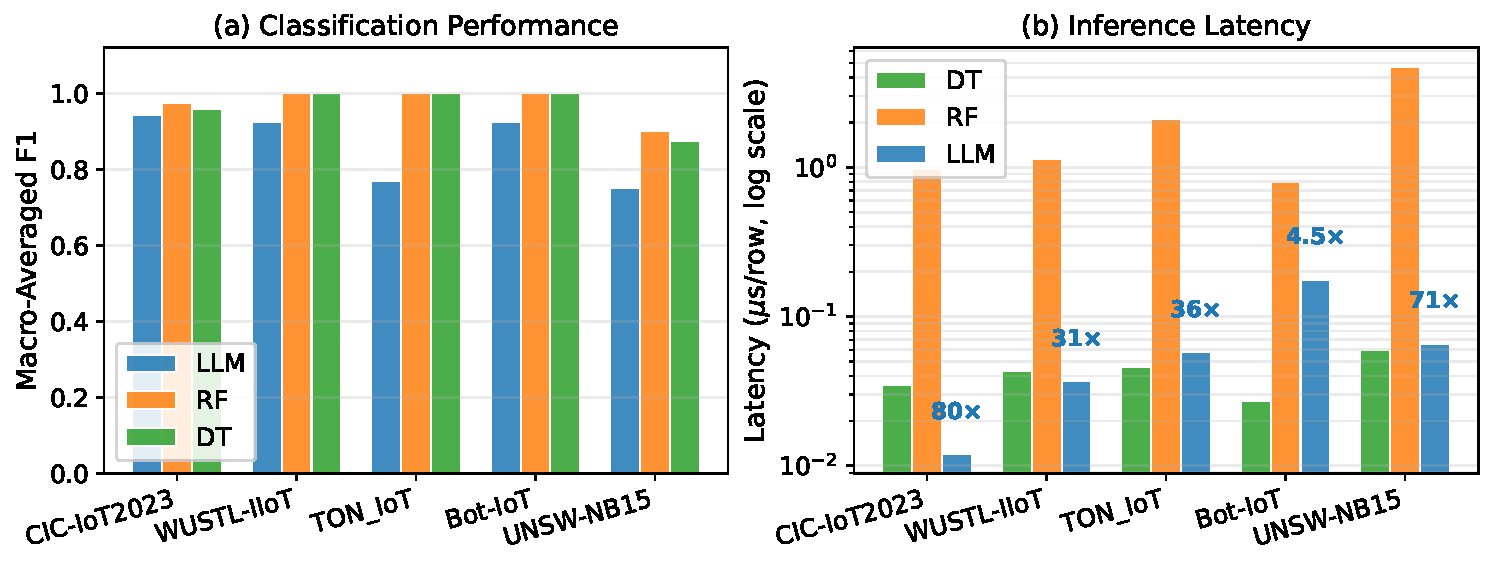
\includegraphics[width=\columnwidth]{figures/fig_comparison_summary.pdf}
  \caption{Binary macro-averaged F1 across all five datasets. LLM values are
    mean over three seeds $\{42, 123, 456\}$ from Table~\ref{tab:policy_refinement},
    best vendor per dataset. RF and DT are binary baselines averaged over ten runs.}
  \label{fig:comparison_summary}
\end{figure}

Fig.~\ref{fig:comparison_summary} summarises the binary F1 comparison.
The LLM policy lies within $0.02$ of Random Forest on four of the five datasets.
The sole substantial gap is UNSW-NB15 (LLM~$0.70$ vs.\ RF~$0.90$), which reflects the structural feature-overlap ceiling discussed in \S\ref{subsec:multiclass_results} rather than a method limitation.
On all other datasets the LLM policy matches gradient classifiers trained on the full feature distribution.

Table~\ref{tab:attack_precision_current} reports attack-class precision,
recall and F1 for both vendors, again as mean over the three-seed campaign.
The pattern is consistent with the macro-F1 trend in
Table~\ref{tab:policy_refinement}: four datasets reach attack F1 $\geq 0.97$
under at least one vendor; TON\_IoT lands at $0.81$ (Haiku) / $0.85$
(Gemini); UNSW-NB15 lands at $0.77$ under both vendors with attack recall
near $0.95$ and the precision-recall tradeoff driven by the structural
feature overlap discussed in \S\ref{subsec:multiclass_results}.

\begin{table}[htbp]
\centering
\caption{Attack-class precision / recall / F1 on the held-out test split.
  Mean over three seeds $\{42, 123, 456\}$. Haiku columns first, then Gemini.}
\label{tab:attack_precision_current}
\begin{tabular}{lcccccc}
\toprule
 & \multicolumn{3}{c}{\textbf{Claude Haiku 4.5}}
 & \multicolumn{3}{c}{\textbf{Gemini 2.5 Flash}} \\
\cmidrule(lr){2-4}\cmidrule(lr){5-7}
\textbf{Dataset} & \textbf{P} & \textbf{R} & \textbf{F1} & \textbf{P} & \textbf{R} & \textbf{F1} \\
\midrule
CIC-IoT2023 & 0.982 & 0.974 & 0.978 & 0.988 & 0.977 & 0.982 \\
WUSTL-IIoT  & 0.978 & 0.983 & 0.980 & 0.974 & 0.997 & 0.986 \\
TON\_IoT    & 0.709 & 0.943 & 0.809 & 0.844 & 0.873 & 0.855 \\
Bot-IoT     & 0.974 & 0.991 & 0.982 & 0.986 & 0.955 & 0.970 \\
UNSW-NB15   & 0.643 & 0.956 & 0.768 & 0.651 & 0.953 & 0.773 \\
\bottomrule
\end{tabular}
\end{table}


The LLM policy generator consistently identifies discriminative thresholds along feature axes that gradient-based importance ranking deprioritises, yielding a detection surface that is complementary to rather than redundant with either baseline. Feature overlap with the RF and DT top-5 is limited across all five datasets (Table~\ref{tab:feature_use_current}). The LLM-selected features concentrate on flow-level timing, connection-state, and address-based descriptors rather than the flag-count and statistical variance features that dominate the tree-based rankings. This divergence is a predictable consequence of how the LLM reasons from representative samples rather than optimising a gradient criterion over the full training distribution.

\begin{table}[htbp]
\centering
\caption{Feature-use comparison: overlap between permutation-importance top-5 for RF and DT versus LLM rule features (standardised evaluation, seed~42). RF$\cap$LLM (DT$\cap$LLM) counts features in common between the respective baseline top-5 and the LLM rule set. LLM Feature Focus summarises the semantic categories of the LLM-selected features.}
\label{tab:feature_use_current}
\begin{tabularx}{\columnwidth}{lXcc}
\toprule
\textbf{Dataset} &
\textbf{LLM Feature Focus} &
\textbf{RF$\cap$LLM} &
\textbf{DT$\cap$LLM} \\
\midrule
CIC-IoT2023 & Flow timing, header length, transport rate & 1 & 0 \\
WUSTL-IIoT  & Source address, packet counts, dest.\ load & 1 & 1 \\
TON\_IoT    & Destination port, connection state, duration & 1 & 2 \\
Bot-IoT     & Source address, port, per-source connection counts & 2 & 2 \\
UNSW-NB15   & Protocol, TTL, connection state, packet counts & 0 & 0 \\
\bottomrule
\end{tabularx}
\end{table}


% ============================================================
\subsection{Threshold Sensitivity Analysis}
\label{subsec:threshold}
%=============================================================

\begin{figure}[t]
    \centering

    \begin{subfigure}[t]{0.5\columnwidth}
        \centering
        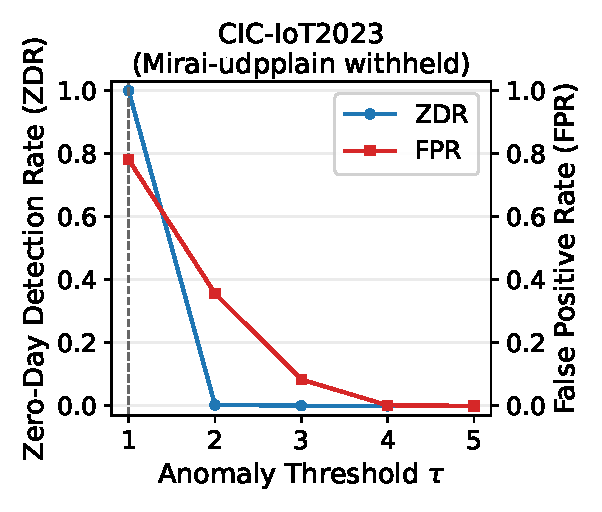
\includegraphics[width=\linewidth]{figures/fig_threshold_cic_mirai.pdf}
        \caption{}
        \label{fig:threshold_mirai}
    \end{subfigure}\hfill
    \begin{subfigure}[t]{0.5\columnwidth}
        \centering
        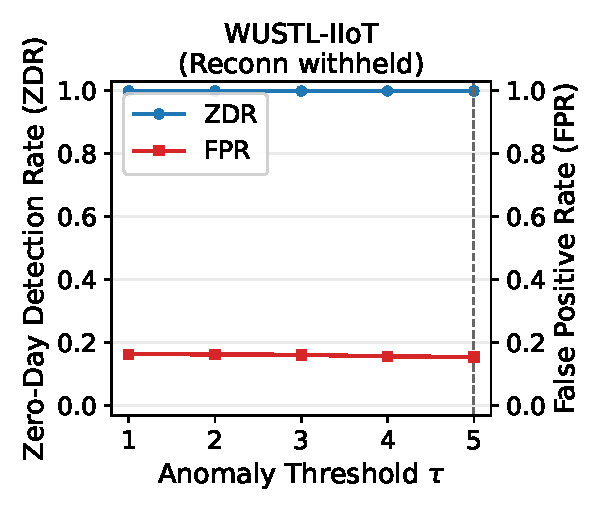
\includegraphics[width=\linewidth]{figures/fig_threshold_wustl.pdf}
        \caption{}
        \label{fig:threshold_wustl}
    \end{subfigure}

    \vspace{0.6em}

    \begin{subfigure}[t]{0.5\columnwidth}
        \centering
        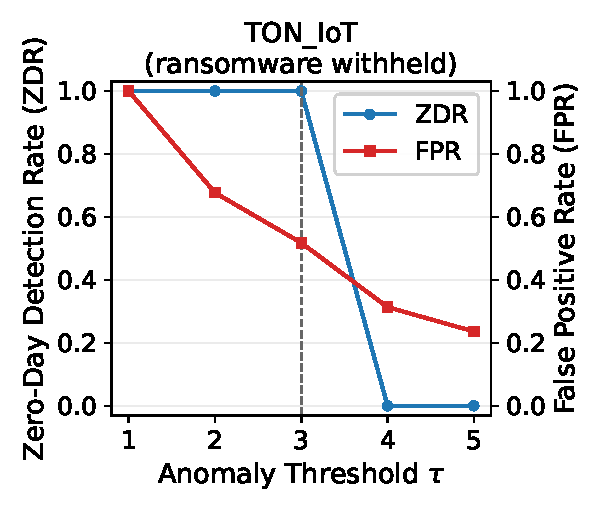
\includegraphics[width=\linewidth]{figures/fig_threshold_toniot.pdf}
        \caption{}
        \label{fig:threshold_toniot}
    \end{subfigure}\hfill
    \begin{subfigure}[t]{0.5\columnwidth}
        \centering
        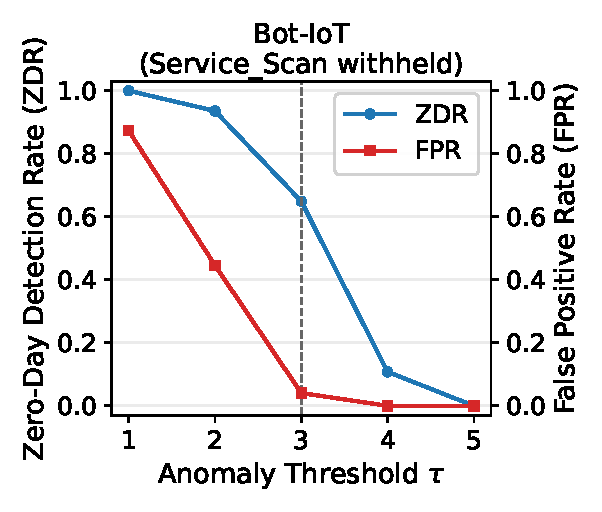
\includegraphics[width=\linewidth]{figures/fig_threshold_botiot.pdf}
        \caption{}
        \label{fig:threshold_botiot}
    \end{subfigure}

    \caption{ZDR and FPR vs.\ anomaly threshold $\tau$ for four
      zero-day withholding scenarios. Dashed vertical line marks the
      operating point maximising ZDR\,$-$\,FPR.
      (a)~CIC-IoT2023, Mirai-udpplain withheld (31{,}864 samples).
      (b)~WUSTL-IIoT, Reconn withheld (8{,}240 samples).
      (c)~TON\_IoT, ransomware withheld (14{,}735 samples).
      (d)~Bot-IoT, Service\_Scan withheld (58{,}626 samples).}
    \label{fig:threshold_sensitivity_all}
\end{figure}

WUSTL-IIoT~(b) and TON\_IoT~(c) are threshold-insensitive successes.
ZDR remains near unity across all $\tau$ while FPR stays below 0.20
even at $\tau=1$, so the operating point choice has no practical
consequence in either case.

Bot-IoT~(d) is the only scenario where $\tau$ constitutes a real
deployment decision. At $\tau=3$ the system achieves ZDR\,$=\,0.65$
with FPR\,$\approx\,0.04$. Tightening to $\tau=4$ drives FPR to
near zero but collapses ZDR to $0.11$.

CIC-IoT2023 with Mirai-udpplain~(a) is a structural failure that no
threshold can resolve. At $\tau=1$ the system flags virtually all
zero-day flows but FPR\,$=\,0.79$. Raising $\tau$ drives ZDR to zero
before FPR reaches an acceptable level. The same pattern holds for
MITM-ArpSpoofing (not shown), confirming this is a dataset-level
property rather than a withheld-class artefact. CIC-IoT2023 sub-variant traffic shares enough statistical signatures with the known training classes that threshold adjustment cannot recover discriminative separation.

% ==============================================================
\subsection{Adversarial Robustness under the Kerckhoffs Assumption}
\label{sec:kerckhoffs}
% ==============================================================

ESR curves are shown in Fig.~\ref{fig:robustness_curves}.

\begin{table}[htbp]
  \centering
  \caption{Median evasion cost ($\varepsilon$@ESR=0.5) under the Kerckhoffs threat
           model (mean over 3 seeds). Higher values indicate harder evasion.}
  \label{tab:kerckhoffs}
  \begin{tabular}{lccccc}
    \toprule
    \textbf{Dataset} & \textbf{LLM\textsubscript{orig}} & \textbf{LLM\textsubscript{anon}} &
    \textbf{DT\textsubscript{d=3}} & \textbf{DT\textsubscript{d=5}} &
    \textbf{RF\textsubscript{d=5}} \\
    \midrule
    CIC-IoT2023 & 0.008 & 0.002 & 0.003 & 0.003 & 0.010 \\
    WUSTL-IIoT  & 0.002 & 0.018 & 0.035 & 0.001 & 0.001 \\
    \bottomrule
  \end{tabular}
\end{table}

\texttt{LLM\textsubscript{orig}} matches \texttt{RF\textsubscript{d=5}} on CIC-IoT2023 ($\varepsilon$@ESR$=0.5$: $0.008$ vs.\ $0.010$), confirming that LLM-generated rules are not inherently more adversarially fragile than trained classifiers. \texttt{DT\textsubscript{d=5}} collapses to ESR${=}1.0$ at $\varepsilon{=}0.001$ on WUSTL-IIoT, 70$\times$ more fragile than \texttt{DT\textsubscript{d=3}}, due to a single \textsc{IdleTime} bottleneck governing 99.97\% of detections. All conditions reach ESR${=}1.0$ at $\varepsilon \leq 0.05$, a structural fragility shared by all conjunctive threshold-based detectors and the motivation for adversarially-aware rule synthesis as future work.

\begin{figure}[htbp]
  \centering
  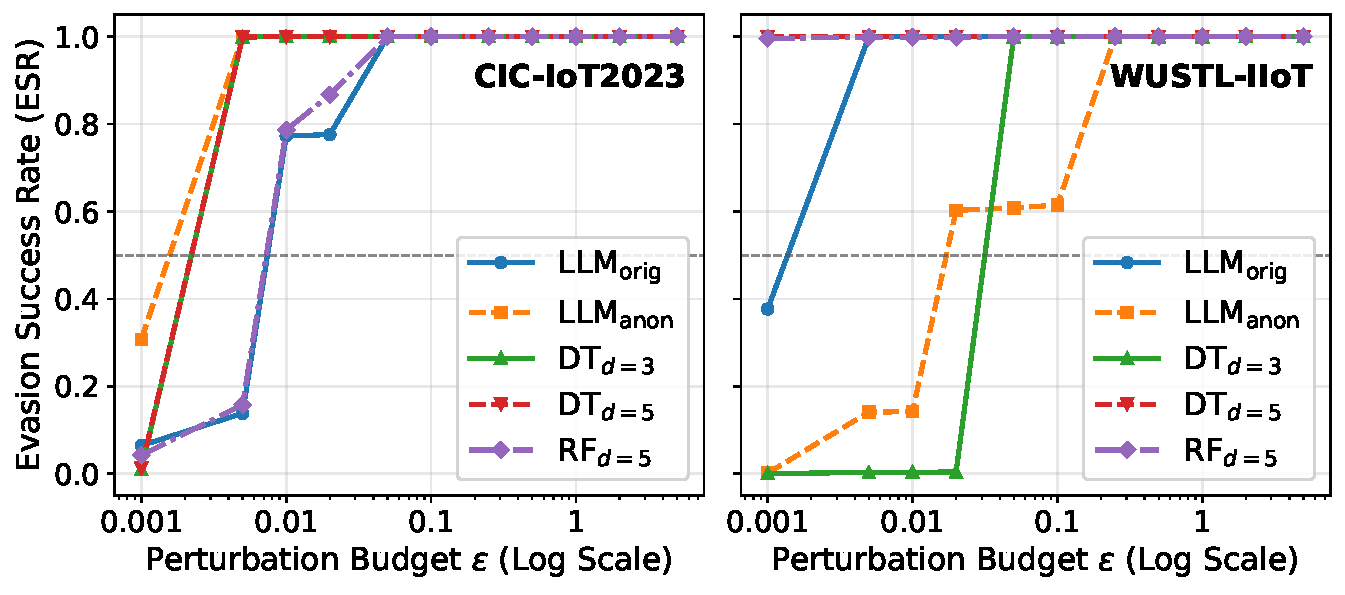
\includegraphics[width=\columnwidth]{figures/fig_robustness_curves.pdf}
  \caption{Evasion success rate (ESR) vs.\ perturbation budget $\varepsilon$ (log scale)
           for all five detection conditions on CIC-IoT2023 (left) and WUSTL-IIoT (right).
           The dashed horizontal line marks ESR=0.5.}
  \label{fig:robustness_curves}
\end{figure}
 
% \begin{figure}[htbp]
%   \centering
%   
\includegraphics[width=\columnwidth]{../iot-llm-hids-pg/experiments/results/kerckhoffs/feature_targeting.png}
%   \caption{Top features targeted by the evasion algorithm at $\varepsilon{=}1.0$.
%            Decision tree conditions collapse to a single bottleneck feature
%            (\texttt{rst\_count} on CIC-IoT2023; \texttt{IdleTime}/\texttt{DIntPkt}
%            on WUSTL-IIoT), whereas LLM and RF conditions distribute perturbations
%            across multiple features.}
%   \label{fig:feature_targeting}
% \end{figure}

% ==============================================================
\subsection{Edge Deployment on Raspberry Pi}
\label{subsec:edge_deployment}
% ==============================================================

The offline stage of the pipeline (LLM inference, embedding model, vector store, and refinement loop) runs on a workstation and produces a compact JSON rule artefact. The edge device receives this artefact and applies it in pure Python to incoming flow-feature rows. Table~\ref{tab:edge_latency} reports the resulting streaming-mode per-row latency on Raspberry Pi~4 (Cortex-A72, 1.8\,GHz) and Raspberry Pi~5 (Cortex-A76, 2.4\,GHz), measured with 30 timed repeats of 1{,}000 rows each. Neither device was thermally throttled during any repeat; both ran at rated frequency throughout. CPU temperature remained below 43\,°C on Pi~4 and below 47\,°C on Pi~5.

\begin{table}[htbp]
\centering
\caption{Streaming-mode median per-row inference latency (ms/flow) on Raspberry Pi~4 and Pi~5
  (30 repeats, active cooling, rated clock). Neither device was throttled during any repeat.}
\label{tab:edge_latency}
\begin{tabular}{lrrr|rrr}
\toprule
 & \multicolumn{3}{c}{\textbf{Raspberry Pi~4}}
 & \multicolumn{3}{c}{\textbf{Raspberry Pi~5}} \\
\cmidrule(lr){2-4}\cmidrule(lr){5-7}
\textbf{Dataset} &
  \textbf{LLM} & \textbf{DT} & \textbf{RF} &
  \textbf{LLM} & \textbf{DT} & \textbf{RF} \\
 & (ms) & (ms) & (ms) & (ms) & (ms) & (ms) \\
\midrule
CIC-IoT2023  & 0.168 & 3.185 & 27.0 & 0.045 & 0.795 & 7.24 \\
WUSTL-IIoT   & 0.173 & 3.520 & 26.9 & 0.048 & 0.888 & 7.15 \\
TON\_IoT     & 0.184 & 3.464 & 26.8 & 0.050 & 0.866 & 7.18 \\
Bot-IoT      & 0.164 & 3.174 & 26.5 & 0.044 & 0.771 & 7.05 \\
UNSW-NB15    & 0.165 & 3.522 & 26.9 & 0.044 & 0.881 & 7.23 \\
\bottomrule
\end{tabular}
\end{table}

The LLM policy is consistently faster than Random Forest by 144$\times$--163$\times$ across both devices and all five datasets, confirming that the macOS latency advantage reported in Table~\ref{tab:timing} transfers in full to resource-constrained ARM hardware. Against Decision Tree, the Pi result diverges sharply from the macOS picture: DT requires 3.2--3.5\,ms per row on Pi~4 and 0.77--0.89\,ms on Pi~5, making the LLM policy 18$\times$--20$\times$ faster than DT on both devices. On macOS ARM the LLM-vs-DT comparison was dataset-dependent, because Apple Silicon's NEON-optimised scikit-learn path eliminates the Python-level tree-traversal overhead that dominates on Raspberry Pi. The LLM policy advantage is therefore \emph{amplified} on embedded ARM hardware: evaluating a flat list of boolean conditions incurs no branch-navigation overhead and requires no hardware-specific linear-algebra tuning. (needs a citation to back this up)

Pi~5 achieves a 3.6$\times$-3.7$\times$ latency reduction relative to Pi~4 across all conditions, consistent with its higher clock frequency and improved Cortex-A76 branch predictor. In batch mode, Pi~5 sustains 612{,}000--1{,}268{,}000 flows per second with the LLM policy artefact, sufficient for high-throughput gateway operation. The peak resident memory footprint is indistinguishable from baseline Python overhead ($\Delta$RSS\,$\approx\,0$\,bytes), as the rule artefact is a compact JSON list requiring no model weights or index structures at inference time. Together, these results confirm that the offline policy-generation cost is incurred once and that the resulting gateway-side runtime is viable on commodity single-board computers.

\subsection{Discussion and Limitations}

Across five IoT benchmark datasets and four experimental axes, four
principal findings emerge.

First, LLM-generated threshold rules achieve near-parity with gradient
classifiers and prior LLM-tuned baselines on datasets with well-separated
traffic signatures (CIC-IoT2023, WUSTL-IIoT, Bot-IoT — all macro F1
$\geq 0.97$, Table~\ref{tab:policy_refinement}), and lift the headline
attack-class F1 on TON\_IoT from $0.37$ in prior single-rule
baselines~\cite{ton_ensemble_2024} to $0.81$--$0.85$ via the
diversity-aware acceptance and weighted-voting layers described in
\S\ref{subsec:policy_generation}. The structural-overlap ceiling on
UNSW-NB15 remains the only case where the prompt-only policy lags deep
fine-tuned baselines, and even there the gap is $0.10$~F1 against models
that require labelled fine-tuning at $10$--$100\times$ the offline
cost~\cite{rulemaster_2025}.

Second, results generalise across LLM vendors. With identical prompts,
acceptance criteria, and voting calibration, Claude Haiku~4.5 and Gemini
2.5~Flash agree to within $0.012$~F1 on four of five datasets; the
single exception is TON\_IoT, where Gemini exceeds Haiku by $0.08$~F1.
The cross-vendor agreement supports the claim that the method's
performance derives from the prompt structure and acceptance scheme
rather than from a single vendor's idiosyncrasies.

Third, removing semantic feature-name information does not degrade, and
in most cases improves detection performance, indicating that the policy
generator operates primarily on numerical sample distributions rather
than name priors.

Fourth, under the Kerckhoffs threat model, LLM-generated rules
distribute evasion cost across multiple features rather than concentrating
it in a single bottleneck, matching or exceeding the adversarial
robustness of comparably complex tree-based baselines.

Together with the edge-deployment latency in \S\ref{subsec:edge_deployment}
($0.044$--$0.184$\,ms/flow on Raspberry Pi~4 and Pi~5 with zero additional
memory footprint at inference), these findings characterise the operating
envelope of RAG-assisted LLM policy generation for IoT intrusion
detection: the approach is competitive with fine-tuned LLM baselines and
gradient classifiers on most benchmarks, vendor-portable, robust under
feature-name obfuscation, and deployable on commodity single-board
computers at sub-millisecond latency without any on-device model weights.

The chief limitation is the structural feature-overlap ceiling on
UNSW-NB15, which affects all classifier families on this dataset and
which the present prompt-only acceptance scheme does not overcome. We
expect that learning a soft per-rule continuous activation (rather than
the boolean fire/no-fire used here) would close part of that gap; we
leave this and the integration of confidence-calibrated soft voting to
future work.
